\part{Using Mana}
\begin{frame}
			 \partpage
\end{frame}

\section[Connecting via Mana Web Portal]{Connecting via Mana Web Portal}
\begin{frame}
\frametitle{Connecting via Mana Web Portal}
\begin{columns}
	\begin{column}{0.46\textwidth}
		\begin{block}{Requirements}
			\begin{itemize}
				\item Valid UH credentials 
				\item Registered for \href{http://www.hawaii.edu/its/uhlogin/}{MFA/DUO}
			\end{itemize}
                        \end{block}
	\end{column}
	\begin{column}{0.46\textwidth}
		\begin{block}{Connection Information}\
	\begin{itemize}
		\item URL: 
		  \begin{itemize} 
		  \item \textbf{https://uhhpc.its.hawaii.edu/}
		  \item \textbf{https://mana.its.hawaii.edu/}
		  \end{itemize}
	\end{itemize}
        \end{block}
	        \end{column}                
	\end{columns}
	\begin{block}{Valid Credentials}\footnotesize
		\begin{itemize}
			\item Your UH user name
			\item Accepted forms of authentication
			\begin{itemize}\scriptsize
				\item UH Password $+$ MFA 
			\end{itemize}
		\end{itemize}
	\end{block}
	\begin{center}\scriptsize
	\end{center}
\end{frame}

\section[Connecting to Mana]{Connecting to Mana}

\subsection[Connecting via Mana Web Portal]{Connecting via Mana Web Portal}
\begin{frame}
\frametitle{Connecting via Mana Web Portal}
 \footnotesize Open OnDemand is an NSF-funded open-source  portal that provides an easy way to access HPC resources.\footnote{\label{OOD}\tiny\ \url{https://openondemand.org/}}
\begin{columns}
	\begin{column}{0.46\textwidth}
		\begin{block}{Requirements}
			\begin{itemize}
				\item Valid UH credentials 
				\item Registered for \href{http://www.hawaii.edu/its/uhlogin/}{MFA/DUO}
			\end{itemize}
                        \end{block}
	\end{column}
	\begin{column}{0.46\textwidth}
		\begin{block}{Connection Information}\
	\begin{itemize}
		  \item \textbf{https://uhhpc.its.hawaii.edu/}
		  \item \textbf{https://mana.its.hawaii.edu/}
		\end{itemize}
        \end{block}
	        \end{column}                
	\end{columns}
	\begin{block}{Valid Credentials}\footnotesize
		\begin{itemize}
			\item Your UH user name
			\item Accepted forms of authentication
			\begin{itemize}\scriptsize
				\item UH Password $+$ MFA 
			\end{itemize}
		\end{itemize}
	\end{block}
	\begin{center}\scriptsize
	\end{center}
 \footnotesize Open OnDemand provides (but it's not limited to): file management, CLI access, job management and monitoring, graphical desktop environments and applications.
\end{frame}

\subsection[Connecting via SSH]{Connecting via SSH}
\begin{frame}
\frametitle{Connecting via SSH}
\begin{columns}
	\begin{column}{0.46\textwidth}
		\begin{block}{Requirements}
			\begin{itemize}
				\item Valid UH credentials 
				\item Registered for \href{http://www.hawaii.edu/its/uhlogin/}{MFA/DUO}
				\item Familiarity with a SSH client \&\\a file-transfer method
				\item Comfortable with the CLI
			\end{itemize}
                        \end{block}
	\end{column}
	\begin{column}{0.46\textwidth}
		\begin{block}{Connection Information}\
	\begin{itemize}
		\item Login node: 
		  \begin{itemize} 
		  \item \textbf{uhhpc.its.hawaii.edu}
		  \end{itemize}
		\item DTNs:
		  \begin{itemize} 
		  \item \textbf{hpc-dtn1.its.hawaii.edu}
		  \item \textbf{hpc-dtn2.its.hawaii.edu}
		  \end{itemize}
	\end{itemize}
        \end{block}
	        \end{column}                
	\end{columns}
	\begin{block}{Valid Credentials}\footnotesize
		\begin{itemize}
			\item Your UH user name
			\item Accepted forms of authentication
			\begin{itemize}\scriptsize
				\item UH Password $+$ MFA 
				\item SSH key $+$ MFA
			\end{itemize}
		\end{itemize}
	\end{block}
	\begin{center}\scriptsize
	\textbf{\large Try and connect to the {\mana} Login node now using your SSH client}
	\end{center}
\end{frame}

 
\section[Directories \& Centralized Software]{Directories \& Centralized Software }
\subsection{User Directories}
\begin{frame}[fragile]
\frametitle{User Directories}
\begin{block}{Filesystem}
\begin{semiverbatim}\tiny \texttt
[testuser@login001 \ctilde]\$ df -h
Filesystem                                       Size  Used Avail Use\%  Mounted on
fs01:/mnt/datastore/hpc/home/testuser             50G  128K   50G   1\%  /home/testuser
fs02:/mnt/datastore/hpc/scratch/testuser         5.0T  256K  5.0T   1\%  /mnt/scratch/nfs_fs02/testuser
10.103.15.230@o2ib,10.103.15.231@o2ib:/scratch    61T  5.1T  55T   9\%   /mnt/scratch/lustre_01
\end{semiverbatim}
\end{block}
\begin{block}{Home}
%lrwxrwxrwx 1 testuser testuser 19 Jan 15 20:38 \textcolor{teal}{lustre_01} -> /mnt/scratch/lustre_01/testuser
\begin{semiverbatim}\tiny \texttt
[testuser@login001 \ctilde]\$ ls -l 
total 1
drwxr-xr-x 3 testuser testuser 23 Jan 15 20:38 examples
lrwxrwxrwx 1 testuser testuser 19 Jan 15 20:38 \textcolor{teal}{nfs_scratch} -> /mnt/scratch/nfs_fs02/testuser
lrwxrwxrwx 1 testuser testuser 19 Jan 15 20:38 \textcolor{teal}{lus_scratch} -> /mnt/scratch/lustre_01/scratch/testuser
\end{semiverbatim}
\end{block}
\begin{itemize}
		\item \ctilde{}/examples contains example scripts to use as templates
		\item \ctilde{}/nfs\_scratch is a symlink to the NFS scratch file system
		\item \ctilde{}/lus\_scratch is a symlink to the lustre scratch file system
\end{itemize}
\end{frame}


\subsection{Modules}
\begin{frame}
	\frametitle{Modules}\footnotesize

	  A tool to help users manage their Unix or Linux shell environment, by allowing groups of related environment-variable settings to be made or removed dynamically.\footnote{\label{wiki_module}\tiny\
             \url{https://en.wikipedia.org/wiki/Environment_Modules_(software)}}
	\begin{block}{Commands}
	  \begin{itemize}\footnotesize
			\item `module avail' -- list installed modules
			\item `module show $<$module name$>$' -- Show what actions a module performs
			\item `module load $<$module name$>$' -- Loads the named module
                        \item `module spider $<$search string$>$' -- search the modules list for a match
                        \item `module list' -- Show what modules are loaded
			\item `module purge' -- Unload all loaded modules
		\end{itemize}
        \end{block}
	\begin{itemize}\footnotesize
                \item Hidden modules can be shown using the \ddash{}show\_hidden flag, e.g., `module \ddash{}show\_hidden avail'
	        \item We create modules for frequently requested software packages for all users to access
		\item Compilers, libraries, interpreters, applications are all added as modules
		\item Users are encouraged to install software in their home/group directories
		\item Modules can be listed on the login nodes, but loaded applications will only work on the compute nodes
                \item {\mana} currently uses \href{https://lmod.readthedocs.io/en/latest/010\_user.html}{lmod}
	\end{itemize}
\end{frame}

\section[Job Scheduler]{Job Scheduler}

\subsection{Terminology}
\begin{frame}
	\frametitle{Terminology}
	\begin{itemize}
          \item \textbf{Job Scheduler} -- A tool/application to control and prioritize the execution order of unrelated jobs 
          \item \textbf{Job} -- Another name for a script or application that is to be executed
          \item \textbf{Job ID} -- A number assigned to each job submitted to the job scheduler
	  \item \textbf{CPU/Socket} -- A processing unit in the node which may contain one or more cores
	  \item \textbf{Core} -- A processing element on a CPU  (Multi-threading)
	  \item \textbf{Task} -- An instance of a running program or process (MPI)
	  \item \textbf{Partition} -- A group of nodes divided into possibly overlapping sets, which also contains constraints for the given set of nodes
            
            %	  \btVFill
            %    \begin{center}On the UH-HPC, you will primarily specify jobs using Cores, Tasks, and the partition.  CPU/Socket are an option is SLURM, but  Please navigate to \textbf{\ctilde/examples/slurm/non-mpi} and try to submit the example batch submission script.\end{center}
	\end{itemize}
\numlessfootnotetxt{\tiny \url{http://slurm.schedmd.com/quickstart.html}}
\end{frame}


\subsection{Slurm}
\begin{frame}
  \frametitle{Slurm Workload Manager}
  {\mana} uses the Slurm Workload Manager to allocate nodes and assign jobs to them
  
  \begin{block}{How it works}
    Jobs are not executed in a \textbf{first in first out} manner.  Instead, jobs are assigned a priority, which is continuously being re-evaluated for pending jobs.
    \\~\\Depending on load, some resources may go idle while waiting for sufficient free resources for a higher priority job.
    In these cases, the scheduler will use what is known as \textbf{backfilling} to fill in the idle machines with jobs that will not affect the start time of higher priority jobs.
	\end{block}
    
       
	\numlessfootnotetxt{\tiny \url{https://en.wikipedia.org/wiki/Slurm_Workload_Manager}}
	\numlessfootnotetxt{\tiny \url{http://slurm.schedmd.com/slurm.html}}
\end{frame}




\subsection{Commands}
\begin{frame}
\frametitle{Commands}
  \begin{block}{Basic}
    \begin{itemize}
    \item \emph{\textbf{sbatch}} -- Used to submit a job script for later execution
    \item \emph{\textbf{srun}} --  Used to submit a job for execution or initiate job steps in real time
    \item \emph{\textbf{scancel}} -- Used to cancel a pending or running job or job step
    \end{itemize}
  \end{block}
  \begin{block}{Informational}
    \begin{itemize}
    \item \emph{\textbf{squeue}} -- Reports the state of jobs or job steps
    \item \emph{\textbf{sinfo}} -- Reports the state of partitions and nodes managed by Slurm
    \item \emph{\textbf{sacct}} -- Reports job accounting information about active or completed jobs
    \end{itemize}
  \end{block}
  
  \begin{itemize}\footnotesize
  \item[--] Examples usage of the Slurm commands can be seen on schedmd's \href{http://slurm.schedmd.com/quickstart.html}{quickstart}
  \end{itemize}
  \numlessfootnotetxt{\tiny \url{http://slurm.schedmd.com/quickstart.html}}
\end{frame}

%% \subsubsection{How jobs are scheduled}
%% \begin{frame}
%% \frametitle{How jobs are scheduled}
%% User submitted jobs are executed one of two ways:
%% \begin{enumerate}
%% \item backfilling
%% \item Priority -- assigned by a  fair share alogrithm
%%   \end{enumerate}
%% Factors such as the following are all used to determine the order in which jobs are executed: 
%% \begin{itemize}
%% \item Runtime
%% \item Amount of resources requested
%% \item Age of job
%% \item Amount of core hours a user has used in recent history
%% \end{itemize}
%% \end{frame}

\subsection {Submitting Jobs}
\subsubsection{Interactive Jobs}
\begin{frame}
  \frametitle{Interactive jobs using srun}

  \begin{block}{Command}\small
		\begin{semiverbatim}$[$login \ctilde$]$\$ srun -I30 -p sandbox -N 1 -c 1 \ddash{}mem=6G -t 0-01:00:00 \ddash{}pty /bin/bash\end{semiverbatim}	
  \end{block}
  \begin{block}{Options}\small
	\begin{itemize}
	\item \textbf{-I30} -- exit if resources are not available within the time period specified (30 seconds)
	\item \textbf{-p sandbox} -- Submit my interactive job to the sandbox partition
	\item \textbf{-N 1} -- Number of nodes requested (If omitted, default is 1)
	\item \textbf{-c 1} -- Number of cores per task requested (If omitted, default is 1)
	\item \textbf{\ddash{}mem$=$6G} --Memory allocated per node (See partition details for defaults)
	\item \textbf{-t 0-01:00:00} -- How much time you are requesting (DD-HH:MM:SS)
	\item \textbf{\ddash{}pty} -- Execute initial task in pseudo terminal mode
	\item \textbf{/bin/bash} -- Task to execute
	\end{itemize}
	\end{block}
  \btVFill
  \begin{center}\small Interactive jobs terminate when the specified time has elapsed or if you give the \textbf{exit} command.\\Interactive jobs are good for testing, compiling and relatively short jobs.\\Longer jobs should use a shell script and \textbf{sbatch}.\\ \end{center}
  \end{frame}


\subsubsection{Batch Jobs}
\begin{frame}
  \frametitle{Batch job using sbatch}
  \begin{block}{Command}
		\begin{semiverbatim}$[$login \ctilde$]$\$ sbatch <path to shell script>\end{semiverbatim}	
  \end{block}
  \begin{block}{Info}
		\begin{itemize}
		\item Where sbatch is executed, becomes the jobs working directory
		\item Submission scripts are shell scripts that begin with special comments that are parameters for the scheduler
		\item Parameters are evaluated with the command-line taking precedent over what the shell script contains
                \item Jobs submitted with sbatch are assigned a job ID by Slurm
		\end{itemize}
	\end{block}
	  \btVFill
  \begin{center}Please navigate to \textbf{\ctilde/examples/slurm/non\_mpi} and try to submit the example batch submission script (non\_mpi.slurm)  using sbatch.\end{center}
\end{frame}


%\begin{frame}[fragile]
%\frametitle{Example Batch Job Script}
%\begin{semiverbatim}\tiny
%[login001 nfs_fs02]\$ cat example.slurm
%
%\#!/bin/bash
%\# Comments (\#) and empty lines are fine between \#SBATCH
%\#SBATCH \ddash{}job-name=example
%\#SBATCH \ddash{}partition=sandbox
%\#SBATCH \ddash{}time=0-04:00:00 ## time format is DD-HH:MM:SS
%\# task-per-node x cpus-per-task should not exceed core count on an individual node 
%\#SBATCH \ddash{}nodes=1
%\#SBATCH \ddash{}tasks-per-node=1
%\#SBATCH \ddash{}cpus-per-task=19
%\#\#SBATCH \ddash{}cpu-specs=0 # Allow access to all cores on a node
%\#SBATCH \ddash{}mem=64G \# Memory per node my job requires
%\#SBATCH \ddash{}distribution="*:*:*" \# set the task and core distribution to the defaults
%\#SBATCH \ddash{}constraint=``x86''
%\#\#SBATCH \ddash{}constraint=``x86\&ib_qdr'' \# Used for MPI jobs that requires inter-node communication via IB
%\#\#SBATCH \ddash{}gres=gpu:NV-K40:2 \# commented out
%\#SBATCH \ddash{}error=example-\%A.err \# \%A - filled with jobid, where to write the stderr
%\#SBATCH \ddash{}output=example-\%A.out \# \%A - filled with jobid, wher to write the stdout
%\#\# Useful for remote notification
%\#SBATCH \ddash{}mail-type=BEGIN,END,FAIL,REQUEUE,TIME\_LIMIT\_80
%\#SBATCH \ddash{}mail-user=user@test.org
%\# All options and environment variables found on schedMD site: \href{http://slurm.schedmd.com/sbatch.html}{http://slurm.schedmd.com/sbatch.html}
%\# =============== Start of commands to execute ===============
%\# source \ctilde/.bash_profile \# Not required unless you need something from your environment
%export OMP\_NUM\_THREADS=\$\{SLURM\_CPUS\_PER\_TASK\}
%module load lang/R  \# load the default R software module
%Rscript hello.r
%\end{semiverbatim}
%\end{frame}




\subsection{Partition Details}
\begin{frame}
\footnotesize
\frametitle{Partitions}
\begin{center}
  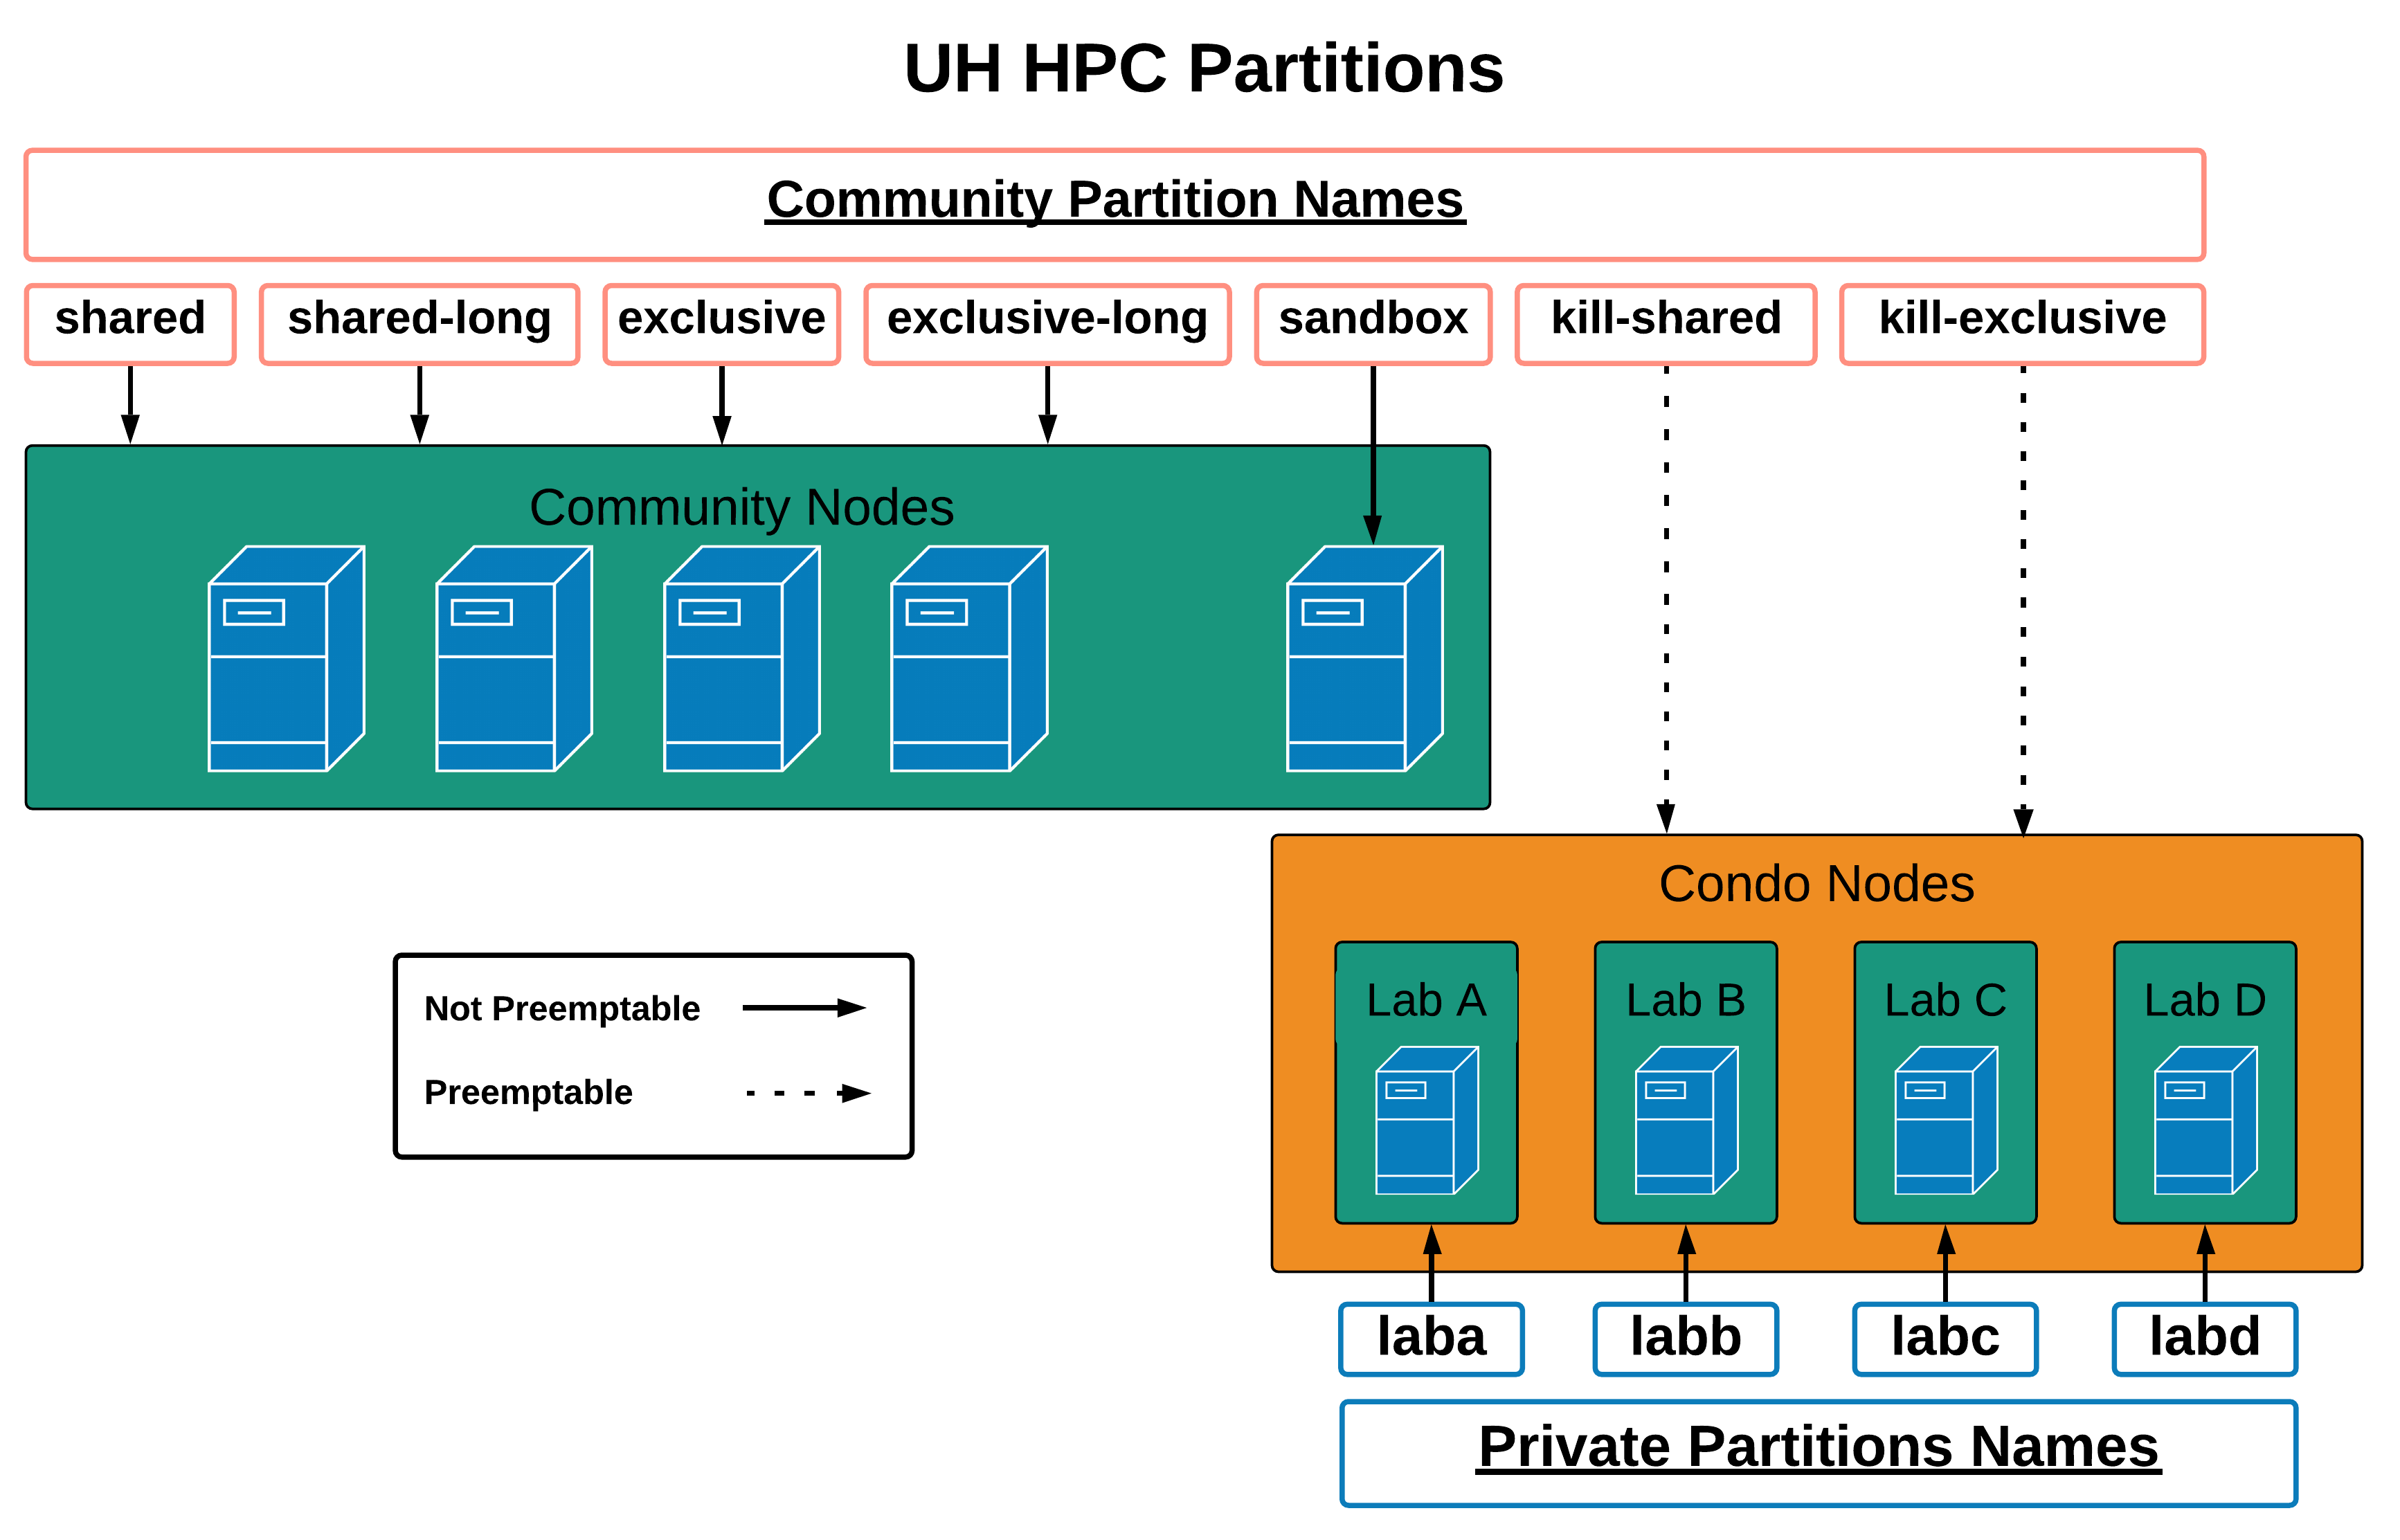
\includegraphics[scale=0.35]{partitions.png}
\end{center}
\end{frame}


\begin{frame}
\footnotesize
\frametitle{Partitions }
\vspace{-10pt}
\begin{block}{\small Details}
\centering
  \resizebox{0.95\textwidth}{!}{%
\begin{tabular}{l || c || c || c || c || c || c }
\toprule                                                                    
\thead{\textbf{Partition}} & \thead{\textbf{Max walltime}} & \thead{\textbf{Jobs - total(running)}} & \thead{\textbf{Max nodes per job}} & \thead{\textbf{Default memory}}& \thead{\textbf{Shared}} & \thead{\textbf{Preemption}}  \\
%\toprule                                                                    
%\toprule                                                                    
\midrule
\midrule
gpu & 3-00:00:00 & $\infty$ & 1 & 512 MB & YES & NO \\
\hline
\hline
gpu-sandbox & 0-04:00:00 & $\infty$(2) & 2 & 512 MB & YES & NO \\
\hline
\hline
sandbox & 0-04:00:00 & $\infty$(2) & 2 & 512 MB & YES & NO \\
\hline
\hline
shared & 3-00:00:00 & $\infty$ & 1 & 512 MB & YES & NO \\
\hline
\hline
shared-long & 7-00:00:00 & 5(2) & 1 & 512 MB & YES & NO \\
\hline
\hline
exclusive & 3-00:00:00 & $\infty$ & 20 & $\infty$ & NO & NO \\
\hline
\hline
exclusive-long & 7-00:00:00 & 5(2) & 20 & $\infty$ & NO & NO \\
\hline
\hline
kill-shared & 3-00:00:00 & $\infty$ & 1 & 512 MB & YES & YES \\
\hline
\hline
kill-exclusive & 3-00:00:00 & $\infty$ & 20 & $\infty$ & NO & YES \\
\bottomrule 
\end{tabular}   
  }

\end{block}

%\vspace{-5pt}
%
%\begin{block}{\small Node Breakdown}
%\centering
  %\resizebox{0.95\textwidth}{!}{%
%\begin{tabular}{l || c || c || c || c || c || c }
%\toprule  
%\thead{\textbf{Partition}} & \thead{\textbf{Intel x86}}  & \thead{\textbf{GPU}} & \thead{\textbf{IB}} & \thead{\textbf{Ethernet}} & \thead{\textbf{Min:Max Cores per node}} & \thead{\textbf{Min:Max Memory per node}\\\textbf{\tiny{(95\% useable)}}} \\
%%\toprule                                                                    
%%\toprule                                                                    
%\midrule
%\midrule
%sandbox & 4 & 0 & 4 & 0 & 20:20 & 128:128 GB \\
%\hline
%\hline
%shared & 152 & 1 & 152 & 0 & 20:40 & 128:1024 GB \\
%\hline
%\hline
%shared-long & 152 & 1 & 152 & 0 & 20:40 & 128:1024 GB \\
%\hline
%\hline
%exclusive & 152 & 1 & 152 & 0 & 20:40 & 128:1024 GB \\
%\hline
%\hline
%exclusive-long & 152 & 1 & 152 & 0 & 20:40 & 128:1024 GB \\
%\hline
%\hline
%kill & 141 & 9 & 133 & 8 & 20:40 & 96:1024 GB \\
%\hline
%\hline
%kill-exclusive & 141 & 9 & 133 & 8 & 20:40 & 96:1024 GB \\
%\bottomrule 
%\end{tabular}   
%}
%
%\end{block}
\end{frame}

\subsection{Constraints \& General Resources}

\begin{frame}
\frametitle{Constraints, General Resources \& Core Specialization}
\vspace{-8pt}
\begin{block}{{\ddash}constraint} Users can select nodes for a job by specifying a value or values for the constraint option. Only nodes having features matching the job constraints will be used to satisfy the request. Multiple constraints may be specified with ``\&'' (AND), ``|'' (OR), etc.
\end{block}
\vspace{-5pt}
\begin{block}{{\ddash}gres} Specifies a comma delimited list of generic consumable resources which a job should be granted access to. 
\end{block}
\vspace{-5pt}
\begin{block}{{\ddash}core-spec}
On {\mana}, the scheduler by default withholds 1 core per node from use by users through a feature in Slurm known as \textbf{core specialization}.  This is done to improve job performance.  This can be overridden by users but is not recommended.
\footnote[1,frame]{\tiny \href{https://slurm.schedmd.com/core_spec.html}{https://slurm.schedmd.com/core\_spec.html}} \footnote[2,frame]{\tiny \href{https://slurm.schedmd.com/SUG14/process_isolation.pdf}{https://slurm.schedmd.com/SUG14/process\_isolation.pdf}}
\end{block}
  \numlessfootnotetxt{\tiny \href{http://go.hawaii.edu/ex2}{Information on Constraints, general resources and node specifications}}
\end{frame}
